% Figure: a tight tile next to the left wall and a slightly tilted pose near it (tilt exaggerated)
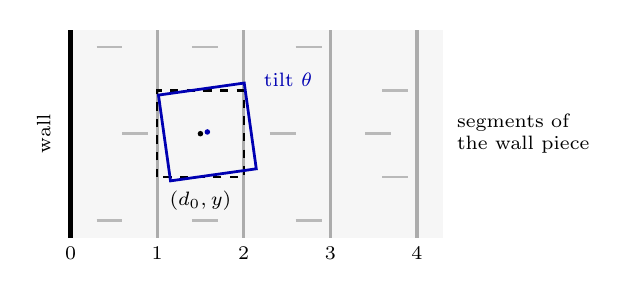
\begin{tikzpicture}[x=1.1cm,y=1.1cm,font=\scriptsize]
  \fill[gray!7] (0,-1.2) rectangle (4.3,1.2);
  \draw[line width=1.5pt] (0,-1.2) -- (0,1.2);
  \node[below] at (0,-1.2) {$0$};
  \foreach \x in {1,2,3,4} {\draw[gray!65,line width=1.1pt] (\x,-1.2) -- (\x,1.2); \node[below] at (\x,-1.2) {$\x$};}
  \foreach \y/\x in {-1/0.3,-1/1.4,-1/2.6,0/0.6,0/2.3,0/3.4,1/0.3,1/1.4,1/2.6,-0.5/3.6,0.5/3.6} \draw[gray!55,line width=0.9pt] (\x,\y) -- ++(0.3,0);
  \draw[dashed,line width=0.9pt] (1,-0.5) rectangle (2,0.5);
  \begin{scope}[shift={(1.58,0.02)},rotate=8]
    \draw[blue!70!black,line width=1pt] (-0.5,-0.5) rectangle (0.5,0.5);
  \end{scope}
  \fill (1.5,0) circle (1pt); \fill[blue!70!black] (1.58,0.02) circle (1pt);
  \node[below] at (1.5,-0.55) {$(d_0,y)$};
  \node[blue!70!black,right] at (2.12,0.62) {tilt $\theta$};
  \node[left,rotate=90,anchor=south] at (-0.12,0) {wall};
  \node[right,align=left] at (4.35,0) {segments of\\the wall piece};
\end{tikzpicture}
